% Options for packages loaded elsewhere
\PassOptionsToPackage{unicode}{hyperref}
\PassOptionsToPackage{hyphens}{url}
%
\documentclass[
  english,
  man,floatsintext]{apa6}
\usepackage{lmodern}
\usepackage{amssymb,amsmath}
\usepackage{ifxetex,ifluatex}
\ifnum 0\ifxetex 1\fi\ifluatex 1\fi=0 % if pdftex
  \usepackage[T1]{fontenc}
  \usepackage[utf8]{inputenc}
  \usepackage{textcomp} % provide euro and other symbols
\else % if luatex or xetex
  \usepackage{unicode-math}
  \defaultfontfeatures{Scale=MatchLowercase}
  \defaultfontfeatures[\rmfamily]{Ligatures=TeX,Scale=1}
\fi
% Use upquote if available, for straight quotes in verbatim environments
\IfFileExists{upquote.sty}{\usepackage{upquote}}{}
\IfFileExists{microtype.sty}{% use microtype if available
  \usepackage[]{microtype}
  \UseMicrotypeSet[protrusion]{basicmath} % disable protrusion for tt fonts
}{}
\makeatletter
\@ifundefined{KOMAClassName}{% if non-KOMA class
  \IfFileExists{parskip.sty}{%
    \usepackage{parskip}
  }{% else
    \setlength{\parindent}{0pt}
    \setlength{\parskip}{6pt plus 2pt minus 1pt}}
}{% if KOMA class
  \KOMAoptions{parskip=half}}
\makeatother
\usepackage{xcolor}
\IfFileExists{xurl.sty}{\usepackage{xurl}}{} % add URL line breaks if available
\IfFileExists{bookmark.sty}{\usepackage{bookmark}}{\usepackage{hyperref}}
\hypersetup{
  pdftitle={Through the eyes of the teacher},
  pdfauthor={Mandy Klatt1 \& Gregor Kachel1},
  pdflang={en-EN},
  pdfkeywords={keywords},
  hidelinks,
  pdfcreator={LaTeX via pandoc}}
\urlstyle{same} % disable monospaced font for URLs
\usepackage{graphicx,grffile}
\makeatletter
\def\maxwidth{\ifdim\Gin@nat@width>\linewidth\linewidth\else\Gin@nat@width\fi}
\def\maxheight{\ifdim\Gin@nat@height>\textheight\textheight\else\Gin@nat@height\fi}
\makeatother
% Scale images if necessary, so that they will not overflow the page
% margins by default, and it is still possible to overwrite the defaults
% using explicit options in \includegraphics[width, height, ...]{}
\setkeys{Gin}{width=\maxwidth,height=\maxheight,keepaspectratio}
% Set default figure placement to htbp
\makeatletter
\def\fps@figure{htbp}
\makeatother
\setlength{\emergencystretch}{3em} % prevent overfull lines
\providecommand{\tightlist}{%
  \setlength{\itemsep}{0pt}\setlength{\parskip}{0pt}}
\setcounter{secnumdepth}{-\maxdimen} % remove section numbering
% Make \paragraph and \subparagraph free-standing
\ifx\paragraph\undefined\else
  \let\oldparagraph\paragraph
  \renewcommand{\paragraph}[1]{\oldparagraph{#1}\mbox{}}
\fi
\ifx\subparagraph\undefined\else
  \let\oldsubparagraph\subparagraph
  \renewcommand{\subparagraph}[1]{\oldsubparagraph{#1}\mbox{}}
\fi
% Manuscript styling
\usepackage{upgreek}
\captionsetup{font=singlespacing,justification=justified}

% Table formatting
\usepackage{longtable}
\usepackage{lscape}
% \usepackage[counterclockwise]{rotating}   % Landscape page setup for large tables
\usepackage{multirow}		% Table styling
\usepackage{tabularx}		% Control Column width
\usepackage[flushleft]{threeparttable}	% Allows for three part tables with a specified notes section
\usepackage{threeparttablex}            % Lets threeparttable work with longtable

% Create new environments so endfloat can handle them
% \newenvironment{ltable}
%   {\begin{landscape}\begin{center}\begin{threeparttable}}
%   {\end{threeparttable}\end{center}\end{landscape}}
\newenvironment{lltable}{\begin{landscape}\begin{center}\begin{ThreePartTable}}{\end{ThreePartTable}\end{center}\end{landscape}}

% Enables adjusting longtable caption width to table width
% Solution found at http://golatex.de/longtable-mit-caption-so-breit-wie-die-tabelle-t15767.html
\makeatletter
\newcommand\LastLTentrywidth{1em}
\newlength\longtablewidth
\setlength{\longtablewidth}{1in}
\newcommand{\getlongtablewidth}{\begingroup \ifcsname LT@\roman{LT@tables}\endcsname \global\longtablewidth=0pt \renewcommand{\LT@entry}[2]{\global\advance\longtablewidth by ##2\relax\gdef\LastLTentrywidth{##2}}\@nameuse{LT@\roman{LT@tables}} \fi \endgroup}

% \setlength{\parindent}{0.5in}
% \setlength{\parskip}{0pt plus 0pt minus 0pt}

% \usepackage{etoolbox}
\makeatletter
\patchcmd{\HyOrg@maketitle}
  {\section{\normalfont\normalsize\abstractname}}
  {\section*{\normalfont\normalsize\abstractname}}
  {}{\typeout{Failed to patch abstract.}}
\patchcmd{\HyOrg@maketitle}
  {\section{\protect\normalfont{\@title}}}
  {\section*{\protect\normalfont{\@title}}}
  {}{\typeout{Failed to patch title.}}
\makeatother
\shorttitle{Visual attention in teaching and learning processes}
\keywords{keywords\newline\indent Word count: X}
\usepackage{lineno}

\linenumbers
\usepackage{csquotes}
\ifxetex
  % Load polyglossia as late as possible: uses bidi with RTL langages (e.g. Hebrew, Arabic)
  \usepackage{polyglossia}
  \setmainlanguage[]{english}
\else
  \usepackage[shorthands=off,main=english]{babel}
\fi

\title{Through the eyes of the teacher}
\author{Mandy Klatt\textsuperscript{1} \& Gregor Kachel\textsuperscript{1}}
\date{}


\authornote{

Add complete departmental affiliations for each author here. Each new line herein must be indented, like this line.

Enter author note here.

Correspondence concerning this article should be addressed to Mandy Klatt, Egelstraße 2a 04103 Leipzig. E-mail: \href{mailto:mandy.klatt@uni-leipzig.de}{\nolinkurl{mandy.klatt@uni-leipzig.de}}

}

\affiliation{\vspace{0.5cm}\textsuperscript{1} University of Leipzig}

\abstract{
One or two sentences providing a \textbf{basic introduction} to the field, comprehensible to a scientist in any discipline.

Two to three sentences of \textbf{more detailed background}, comprehensible to scientists in related disciplines.

One sentence clearly stating the \textbf{general problem} being addressed by this particular study.

One sentence summarizing the main result (with the words ``\textbf{here we show}'' or their equivalent).

Two or three sentences explaining what the \textbf{main result} reveals in direct comparison to what was thought to be the case previously, or how the main result adds to previous knowledge.

One or two sentences to put the results into a more \textbf{general context}.

Two or three sentences to provide a \textbf{broader perspective}, readily comprehensible to a scientist in any discipline.
}



\begin{document}
\maketitle

\hypertarget{state-of-research}{%
\section{State of research}\label{state-of-research}}

Teaching and classroom management are multidimensional settings in which teachers have to respond immediately to events as they develop (Barnes, 2004). The different interests and abilities of students must be managed in a way that maximizes the active learning time of students and minimizes disruptions whilst teaching. Learning to develop such classroom management skills and to teach effectively is a complicated and complex process (Wolff, Jarodzka, \& Boshuizen, 2017).

During teaching, teachers must be able to select from a variety of visual and acoustic impressions to focus their attention on the essential and to distinguish between relevant and irrelevant events. This ability is called professional vision and is a key component of teacher expertise and successful teaching (Barth, 2017). Eye tracking technology has become a reliable means to study teachers' visual focus of attention (Bogert, 2016; Pouta, Lehtinen, \& Palonen, 2020; Wolff et al., 2017)

Educational research has repeatedly shown that there are differences between experienced and novice teachers in terms of perception and behavioral competencies (Barth, 2017; Bogert, 2016; Wolff et al., 2017). For example, experts direct their attention more often and more evenly to all students, whereas novices only direct their attention to some students. The frequency and duration of fixations as eye movement are decisive (Stuermer, Seidel, Mueller, Häusler, \& Cortina, 2017). Mobile eye-tracking technology has also shown that experienced teachers distribute their focus more efficiently to solve tasks (Jarodzka, Scheiter, Gerjets, \& Van Gog, 2010). Furthermore, in contrast to novices, experts are able to focus their attention on the entire class and guide the class while giving feedback to individual students and answering questions (Cortina, Miller, McKenzie, \& Epstein, 2015).

Hey Mandy, hier wollte ich dir mal zeigen wie man Bilder in papaja einbindet. Viel Spass damit. Ein Beispiel für Tabellen und Graphen machen wir auch zeitnah.



\begin{figure}

{\centering 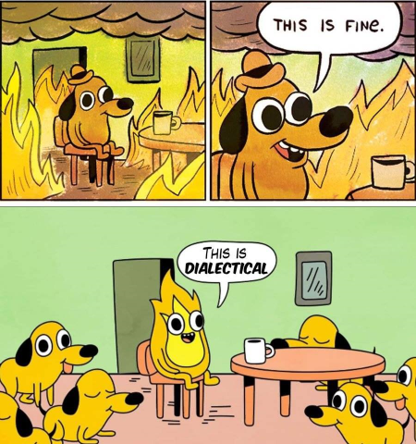
\includegraphics{./pictures/thisisdialectical} 

}

\caption{Illustration of comic material that made the second author of this paper chuckle a bit. For advice on how to insert images, please see the code chunk.}\label{fig:dialectical}
\end{figure}

\hypertarget{research-questions}{%
\subsection{Research questions}\label{research-questions}}

The first study is a laboratory study that uses a quasi-experimental cross-sectional study design to investigate whether the experience of teachers has an influence on the perception of and response to disruptions. The disturbances are experimentally varied using a previously written script. Thus, the aim is to find out whether differences in the allocation of attention between expertise groups can be detected in this controlled context.

In order to answer this question, the hypothesis was formulated that teachers with more professional experience not only notice more disturbances but also notice them faster. In the hypothesis, therefore, it is necessary to check what has already been shown in the research literature: In complex teaching situations, experts have a more structured and elaborate professional knowledge than novices in order to perceive and interpret relevant events and to act appropriately (Berliner, 2001; Lachner, Jarodzka, \& Nückles, 2016).

\hypertarget{methods}{%
\section{Methods}\label{methods}}

We report how we determined our sample size, all data exclusions (if any), all manipulations, and all measures in the study.

\hypertarget{participants}{%
\subsection{Participants}\label{participants}}

For the sample recruitment of the subjects (N = 48, experts n = 24, novices n = 24), schools in the city of Leipzig in Saxony were contacted. The institutions as well as the subjects were informed in detail about the aim and intention of the dissertation project in advance. Participation in the study was voluntary and only took place after written consent has been given.

The selection of the subjects was based on extreme groups, whereby professional experience is the crucial criterion for the selection of experts or novices. Novices were recruited as teachers who have been working in the teaching profession for no more than 3 years, whereas experts were considered to have professional experience of 10 years or more (Messner \& Reusser, 2000).

\hypertarget{procedure}{%
\subsection{Procedure}\label{procedure}}

For this study, lesson units of n = 24 experts and n = 24 novices were recorded by the mobile laboratory of the Department of Empirical School and Classroom Research at the University of Leipzig. The two extreme groups were each divided into groups of four, with one group being invited on each of six different dates. All participants were asked to hold a 15-minute lesson. The duration of each appointment was approximately 2h30min: per extreme group 4 x 15min briefing, 15min lesson units, 10min technical preparation and follow-up and 5min buffer/break.

One person from the group of 4 acted as a teacher, the other three subjects acted as the class. The subjects, who represented the class, were given behavioral instructions in a pre-written script to simulate typical events and disturbances in the classroom (e.g.~putting their heads on the table, chatting, looking at their mobile phones, etc.).

The lesson disturbances were displayed as instructions during the lesson for all \enquote{students} but not the teacher. In order to avoid learning effects, the disruptions in each lesson were distributed pseudo-randomly over the short teaching phase. In addition, the order of the data collection was taken into account in the analyses and variance caused by order was controlled.

By using mobile eye-trackers, the gaze and behavior of the experts and novices was recorded during the lesson. In addition, what the participating teachers said was recorded with a portable microphone. Other sounds and voices were recorded with an audio recorder installed in the middle of the laboratory. Movements, facial expressions and gestures of the subjects were recorded by four cameras from different angles. One camera was installed to film the class from the side. Two more cameras were installed on the blackboard and at the end of the laboratory to film the teacher and class from the front and back. In addition, it the fourth camera was installed in such a way that only facial expressions and gestures of the teacher were recorded, which enables a semi-automated analysis of the movement sequences.

The lessons recorded on video were coded in a post-hoc procedure with a coding software by previously trained raters. The statistical data have been analyzed by using the program RStudio {[}Link: \url{https://rstudio.com/}{]}.

\hypertarget{measures}{%
\subsection{Measures}\label{measures}}

\hypertarget{eye-tracking-equipment}{%
\subsubsection{Eye-tracking equipment}\label{eye-tracking-equipment}}

A binocular Tobii Pro Glasses 2 eye-tracker consisting of a wearable head unit and a recording unit was used to record the eye movements. The head unit is a measuring device with different sensitive sensors. A high-definition scene camera captures a full HD video and an integrated microphone records the surrounding sounds. Infrared light illuminators support the eye tracking sensors which record the eye orientation. The videos were recorded with a sampling rate of 50 Hz and a video resolution with 1920 x 1080 at 25 frames per second. The scene camera has a field of view of 90 deg. in 16:9 format (82 deg. horizontal and 52 deg. vertical) and has a frame dimension of 179 x 159 x 57mm (width x depth x height). The Tobii Pro Glasses Controller software was used to record and calibrate the eye movements.

The Tobii Pro Glasses 2 software allows for non-screen based recordings of a participants' attention while moving in real-world settings. The recordings of the glasses contain both HD-video from the subject's perspective as well as the respective gaze data mapped onto the video. In order to map multiple recordings to AOIs, it is necessary to import the eye-tracking recordings into the Tobii Pro Analyzer software. Also, it is necessary to create a reference image of the scene in which one wishes to plot the gaze data (i.e.~snapshot). Once the snapshot is imported, the gaze recordings of multiple recordings can be mapped to the reference image and analyzed in aggregated form. Tobii Pro does not allow to do AOI based analyses within Pro Lab. Also, the dependency on snapshot reference images makes this approach impractical when working in different settings, i.e.~different classrooms with various participants. Finally, mapping gaze to people or any moving objects complicated the analyses further.

\hypertarget{data-analysis}{%
\subsection{Data analysis}\label{data-analysis}}

We used R (Version 4.0.2; R Core Team, 2019) and the R-packages \emph{papaja} (Version 0.1.0.9997; Aust \& Barth, 2020), and \emph{papayar} (Muschelli, 2016) for all our analyses.

Lorem ipsum dolor sit amet, consetetur sadipscing elitr, sed diam nonumy eirmod tempor invidunt ut labore et dolore magna aliquyam erat, sed diam voluptua. At vero eos et accusam et justo duo dolores et ea rebum. Stet clita kasd gubergren, no sea takimata sanctus est Lorem ipsum dolor sit amet. Lorem ipsum dolor sit amet, consetetur sadipscing elitr, sed diam nonumy eirmod tempor invidunt ut labore et dolore magna aliquyam erat, sed diam voluptua. At vero eos et accusam et justo duo dolores et ea rebum. Stet clita kasd gubergren, no sea takimata sanctus est Lorem ipsum dolor sit amet.

\hypertarget{results}{%
\section{Results}\label{results}}

Lorem ipsum dolor sit amet, consetetur sadipscing elitr, sed diam nonumy eirmod tempor invidunt ut labore et dolore magna aliquyam erat, sed diam voluptua. At vero eos et accusam et justo duo dolores et ea rebum. Stet clita kasd gubergren, no sea takimata sanctus est Lorem ipsum dolor sit amet. Lorem ipsum dolor sit amet, consetetur sadipscing elitr, sed diam nonumy eirmod tempor invidunt ut labore et dolore magna aliquyam erat, sed diam voluptua. At vero eos et accusam et justo duo dolores et ea rebum. Stet clita kasd gubergren, no sea takimata sanctus est Lorem ipsum dolor sit amet.

\hypertarget{discussion}{%
\section{Discussion}\label{discussion}}

Lorem ipsum dolor sit amet, consetetur sadipscing elitr, sed diam nonumy eirmod tempor invidunt ut labore et dolore magna aliquyam erat, sed diam voluptua. At vero eos et accusam et justo duo dolores et ea rebum. Stet clita kasd gubergren, no sea takimata sanctus est Lorem ipsum dolor sit amet. Lorem ipsum dolor sit amet, consetetur sadipscing elitr, sed diam nonumy eirmod tempor invidunt ut labore et dolore magna aliquyam erat, sed diam voluptua. At vero eos et accusam et justo duo dolores et ea rebum. Stet clita kasd gubergren, no sea takimata sanctus est Lorem ipsum dolor sit amet.

\newpage

\hypertarget{references}{%
\section{References}\label{references}}

\begingroup
\setlength{\parindent}{-0.5in}
\setlength{\leftskip}{0.5in}

\hypertarget{refs}{}
\leavevmode\hypertarget{ref-R-papaja}{}%
Aust, F., \& Barth, M. (2020). \emph{papaja: Create APA manuscripts with R Markdown}. Retrieved from \url{https://github.com/crsh/papaja}

\leavevmode\hypertarget{ref-barnes2004significance}{}%
Barnes, D. (2004). The significance of teachers' frames for teaching. In \emph{Teachers and teaching} (pp. 16--38). Routledge.

\leavevmode\hypertarget{ref-barth2017professionelle}{}%
Barth, V. L. (2017). \emph{Professionelle wahrnehmung von störungen im unterricht}. Springer.

\leavevmode\hypertarget{ref-berliner2001learning}{}%
Berliner, D. C. (2001). Learning about and learning from expert teachers. \emph{International Journal of Educational Research}, \emph{35}(5), 463--482.

\leavevmode\hypertarget{ref-bogert2016visualperception}{}%
Bogert, N. J. van den. (2016). \emph{On teachers' visual perception and interpretation of classroom events using eye tracking and collaborative tagging methodologies}. Technische Universiteit Eindhoven.

\leavevmode\hypertarget{ref-cortina2015low}{}%
Cortina, K. S., Miller, K. F., McKenzie, R., \& Epstein, A. (2015). Where low and high inference data converge: Validation of class assessment of mathematics instruction using mobile eye tracking with expert and novice teachers. \emph{International Journal of Science and Mathematics Education}, \emph{13}(2), 389--403.

\leavevmode\hypertarget{ref-jarodzka2010eyes}{}%
Jarodzka, H., Scheiter, K., Gerjets, P., \& Van Gog, T. (2010). In the eyes of the beholder: How experts and novices interpret dynamic stimuli. \emph{Learning and Instruction}, \emph{20}(2), 146--154.

\leavevmode\hypertarget{ref-lachner2016makes}{}%
Lachner, A., Jarodzka, H., \& Nückles, M. (2016). What makes an expert teacher? Investigating teachers' professional vision and discourse abilities. \emph{Instructional Science}, \emph{44}(3), 197--203.

\leavevmode\hypertarget{ref-messner2000berufliche}{}%
Messner, H., \& Reusser, K. (2000). Die berufliche entwicklung von lehrpersonen als lebenslanger prozess. \emph{Beiträge Zur Lehrerinnen-Und Lehrerbildung}, \emph{18}(2), 157--171.

\leavevmode\hypertarget{ref-R-papayar}{}%
Muschelli, J. (2016). \emph{Papayar: View medical research images using the papaya javascript library}. Retrieved from \url{https://CRAN.R-project.org/package=papayar}

\leavevmode\hypertarget{ref-pouta2020student}{}%
Pouta, M., Lehtinen, E., \& Palonen, T. (2020). Student teachers' and experienced teachers' professional vision of students' understanding of the rational number concept.

\leavevmode\hypertarget{ref-R-base}{}%
R Core Team. (2019). \emph{R: A language and environment for statistical computing}. Vienna, Austria: R Foundation for Statistical Computing. Retrieved from \url{https://www.R-project.org/}

\leavevmode\hypertarget{ref-stuermer2017eye}{}%
Stuermer, K., Seidel, T., Mueller, K., Häusler, J., \& Cortina, K. S. (2017). What is in the eye of preservice teachers while instructing? An eye-tracking study about attention processes in different teaching situations. \emph{Zeitschrift Für Erziehungswissenschaft}, \emph{20}(1), 75--92.

\leavevmode\hypertarget{ref-wolff2017see}{}%
Wolff, C. E., Jarodzka, H., \& Boshuizen, H. P. (2017). See and tell: Differences between expert and novice teachers' interpretations of problematic classroom management events. \emph{Teaching and Teacher Education}, \emph{66}, 295--308.

\endgroup


\end{document}
